\documentclass{article}

%Page format
\usepackage{pdfpages}
\usepackage{fancyhdr}
\usepackage[margin=1in]{geometry}

%Math packages and custom commands
\usepackage{algpseudocode}
\usepackage{amsthm}
\usepackage{framed}
\usepackage{hyperref}
\usepackage{tikz}
\usepackage[utf8]{inputenc}
\usepackage[margin=1in]{geometry}
\usepackage{mathtools,amsthm}
\usepackage{enumitem,amssymb}
\newtheoremstyle{case}{}{}{}{}{}{:}{ }{}
\theoremstyle{case}
\newtheorem{case}{Case}
\DeclareMathOperator{\R}{\mathbb{R}}
\DeclareMathOperator{\E}{\mathbb{E}}
\DeclareMathOperator{\Var}{\text{Var}}
\DeclareMathOperator{\Cov}{\text{Cov}}
\newcommand{\bvec}[1]{\mathbf{#1}}
\renewcommand{\P}{\mathbb{P}}
\newcommand{\norm}[2][2]{\| #2\|_{#1}}

\definecolor{shadecolor}{gray}{0.9}

\theoremstyle{definition}
\newtheorem*{answer}{Answer}
\newcommand{\note}[1]{\noindent{[\textbf{NOTE:} #1]}}
\newcommand{\hint}[1]{\noindent{[\textbf{HINT:} #1]}}
\newcommand{\recall}[1]{\noindent{[\textbf{RECALL:} #1]}}
\newcommand{\expect}[1]{\noindent{[\textbf{What we expect:} #1]}}
\newcommand{\mysolution}[1]{\noindent{\begin{shaded}\textbf{Your Solution:}\ #1 \end{shaded}}}

\newlist{todolist}{itemize}{2}
\setlist[todolist]{label=$\square$}
\usepackage{pifont}
\newcommand{\cmark}{\ding{51}}%
\newcommand{\xmark}{\ding{55}}%
\newcommand{\done}{\rlap{$\square$}{\raisebox{2pt}{\large\hspace{1pt}\cmark}}%
\hspace{-2.5pt}}
\newcommand{\wontfix}{\rlap{$\square$}{\large\hspace{1pt}\xmark}}


\title{CS 236 Homework 3 }

\begin{document}
\maketitle

\begin{center}
\begin{tabular}{rl}
Instructor: & Stefano Ermon (ermon@cs.stanford.edu)\\
SUNet ID: & \texttt{anuj42} \\
Name: & Anuj Shetty\\
Collaborators: & 
\end{tabular}
\end{center}

\textit{By turning in this assignment, I agree by the Stanford honor code and declare
that all of this is my own work.} \\

Available: 11/06/2023; Due: 23:59 PST, 11/27/2023

Submission Instructions: Please package all of the programming parts (1.1, 1.2, 1.3, 2.2, 4.2, and 5.5) together using make\_submission.sh and submit the resulting ZIP file on GradeScope.

\section*{Problem 1: Flow models (25 points)}
In this problem, we will implement a Masked Autoregressive Flow (MAF) model on the Moons dataset, where we define $p_{\text {data }}(\boldsymbol{x})$ over a 2 -dimensional space $\left(\boldsymbol{x} \in \mathbb{R}^{n}\right.$ where $\left.n=2\right)$. Recall that MAF is comprised of Masked Autoregressive Distribution Estimator (MADE) blocks, which has a special masking scheme at each layer such that the autoregressive property is preserved. In particular, we consider a Gaussian autoregressive model:

$$
p(\boldsymbol{x})=\prod_{i=1}^{n} p\left(x_{i} \mid \boldsymbol{x}_{<i}\right)
$$

such that the conditional Gaussians $p\left(x_{i} \mid \boldsymbol{x}_{<i}\right)=\mathcal{N}\left(x_{i} \mid \mu_{i},\left(\exp \left(\alpha_{i}\right)^{2}\right)\right)$ are parameterized by neural networks $\mu_{i}=f_{\mu_{i}}\left(\boldsymbol{x}_{<i}\right)$ and $\alpha_{i}=f_{\alpha_{i}}\left(\boldsymbol{x}_{<i}\right)$. Note that $\alpha_{i}$ denotes the log standard deviation of the Gaussian $p\left(x_{i} \mid \boldsymbol{x}_{<i}\right)$. As seen in lecture, a normalizing flow uses a series of deterministic and invertible mappings $f: \mathbb{R}^{n} \rightarrow \mathbb{R}^{n}$ such that $x=f(z)$ and $z=f^{-1}(x)$ to transform a simple prior distribution $p_{z}$ (e.g. isotropic Gaussian) into a more expressive one. In particular, a normalizing flow which composes $k$ invertible transformations $\left\{f_{j}\right\}_{j=1}^{k}$ such that $\boldsymbol{x}=f^{k} \circ f^{k-1} \circ \cdots \circ f^{1}\left(\boldsymbol{z}_{0}\right)$ takes advantage of the change-of-variables property:

$$
\log p(\boldsymbol{x})=\log p_{z}\left(f^{-1}(\boldsymbol{x})\right)+\sum_{j=1}^{k} \log \left|\operatorname{det}\left(\frac{\partial f_{j}^{-1}\left(\boldsymbol{x}_{j}\right)}{\partial \boldsymbol{x}_{j}}\right)\right|
$$

In MAF, the forward mapping is: $x_{i}=\mu_{i}+z_{i} \cdot \exp \left(\alpha_{i}\right)$, and the inverse mapping is: $z_{i}=\left(x_{i}-\mu_{i}\right) / \exp \left(\alpha_{i}\right)$. The $\log$ of the absolute value of the Jacobian is:

$$
\log \left|\operatorname{det}\left(\frac{\partial f^{-1}}{\partial \boldsymbol{x}}\right)\right|=-\sum_{i=1}^{n} \alpha_{i}
$$

where $\mu_{i}$ and $\alpha_{i}$ are as defined above.

Your job is to implement and train a 5-layer MAF model on the Moons dataset for 100 epochs by modifying the MADE and MAF classes in the flow\_network.py file. Note that we have provided an implementation of the sequential-ordering masking scheme for MADE.

\begin{enumerate}
  \item [ 5 points] Implement the forward function in the MADE class in codebase/flow\_network.py. The forward pass describes the mapping $x_{i}=\mu_{i}+z_{i} \cdot \exp \left(\alpha_{i}\right)$.

\mysolution{
        Refer to code submission. 
    }
    

  \item [5 points] Implement the inverse function in the MADE class in codebase/flow\_network.py. The inverse pass describes the mapping $z_{i}=\left(x_{i}-\mu_{i}\right) / \exp \left(\alpha_{i}\right)$

\mysolution{
        Refer to code submission. 
    }
    

  \item [10 points] Implement the log\_probs function in the MAF class in codebase/flow\_network.py. Then train the MAF model for 50 epochs by executing python run\_flow.py. [Hint: you should be getting a validation/test loss of around -1.2 nats]

  \mysolution{
        Refer to code submission. 
    }
    

  \item [ $\mathbf{5}$ points] Visualize 1000 samples drawn the model after is has been trained, which you can do by finding the figure in maf/samples\_epoch50.png. Attach this figure in your writeup - your samples will not be perfect, but should for the most part resemble the shape of the original dataset.

\mysolution{
  
    }

    \begin{figure}[h]
      \centering
      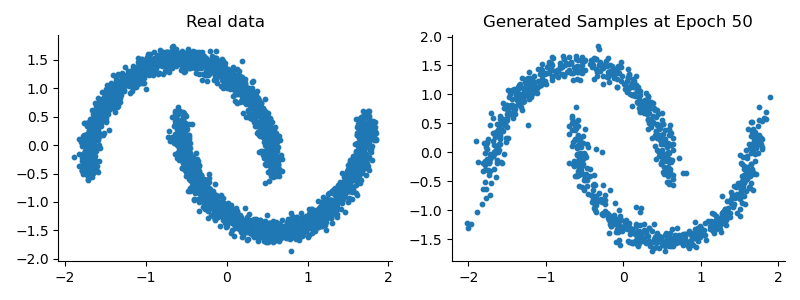
\includegraphics[width=\linewidth]{maf/samples_epoch50.png}
      %\caption{Graphical model for SSVAE. Gray nodes denote observed variables.}
      \label{fig:maf}
  \end{figure}

\end{enumerate}

\section*{Problem 2: Generative adversarial networks (20 points)}
In this problem, we will implement a generative adversarial network (GAN) that models a high-dimensional data distribution $p_{\text {data }}(\boldsymbol{x})$, where $\boldsymbol{x} \in \mathbb{R}^{n}$. To do so, we will define a generator $G_{\theta}: \mathbb{R}^{k} \rightarrow \mathbb{R}^{n}$; we obtain samples from our model by first sampling a $k$-dimensional random vector $\boldsymbol{z} \sim \mathcal{N}(0, I)$ and then returning $G_{\theta}(\boldsymbol{z})$.

We will also define a discriminator $D_{\phi}: \mathbb{R}^{n} \rightarrow(0,1)$ that judges how realistic the generated images $G_{\theta}(\boldsymbol{z})$ are, compared to samples from the data distribution $x \sim p_{\text {data }}(\boldsymbol{x})$. Because its output is intended to be interpreted as a probability, the last layer of the discriminator is frequently the sigmoid function,

$$
\sigma(x)=\frac{1}{1+e^{-x}},
$$

which constrains its output to fall between 0 and 1 . For convenience, let $h_{\phi}(\boldsymbol{x})$ denote the activation of the discriminator right before the sigmoid layer, i.e. let $D_{\phi}(\boldsymbol{x})=\sigma\left(h_{\phi}(\boldsymbol{x})\right)$. The values $h_{\phi}(\boldsymbol{x})$ are also called the discriminator's logits.

There are several common variants of the loss functions used to train GANs. They can all be described as a procedure where we alternately perform a gradient descent step on $L_{D}(\phi ; \theta)$ with respect to $\phi$ to train the discriminator $D_{\phi}$, and a gradient descent step on $L_{G}(\theta ; \phi)$ with respect to $\theta$ to train the generator $G_{\theta}$ :

$$
\min _{\phi} L_{D}(\phi ; \theta), \quad \min _{\theta} L_{G}(\theta ; \phi)
$$

In lecture, we talked about the following losses, where the discriminator's loss is given by

$$
L_{D}(\phi ; \theta)=-\mathbb{E}_{\boldsymbol{x} \sim p_{\mathrm{data}}(\boldsymbol{x})}\left[\log D_{\phi}(\boldsymbol{x})\right]-\mathbb{E}_{\boldsymbol{z} \sim \mathcal{N}(0, I)}\left[\log \left(1-D_{\phi}\left(G_{\theta}(\boldsymbol{z})\right)\right)\right]
$$

and the generator's loss is given by the minimax loss

$$
L_{G}^{\operatorname{minimax}}(\theta ; \phi)=\mathbb{E}_{\boldsymbol{z} \sim \mathcal{N}(0, I)}\left[\log \left(1-D_{\phi}\left(G_{\theta}(\boldsymbol{z})\right)\right)\right]
$$

\begin{enumerate}
  \item [5 points] Unfortunately, this form of loss for $L_{G}$ suffers from a vanishing gradient problem. In terms of the discriminator's logits, the minimax loss is
\end{enumerate}

$$
L_{G}^{\operatorname{minimax}}(\theta ; \phi)=\mathbb{E}_{\boldsymbol{z} \sim \mathcal{N}(0, I)}\left[\log \left(1-\sigma\left(h_{\phi}\left(G_{\theta}(\boldsymbol{z})\right)\right)\right)\right]
$$

Show that the derivative of $L_{G}^{\operatorname{minimax}}$ with respect to $\theta$ is approximately 0 if $D\left(G_{\theta}(\boldsymbol{z})\right) \approx 0$, or equivalently, if $h_{\phi}\left(G_{\theta}(\boldsymbol{z})\right) \ll 0$. You may use the fact that $\sigma^{\prime}(x)=\sigma(x)(1-\sigma(x))$. Why is this problematic for the training of the generator when the discriminator successfully identifies a fake sample $G_{\theta}(\boldsymbol{z})$ ?

\mysolution{

Given the minimax loss for the generator \(L_{G}^{\text{minimax}}(\theta; \phi)\):
\[ L_{G}^{\text{minimax}}(\theta; \phi) = \mathbb{E}_{z \sim \mathcal{N}(0,I)}[\log(1 - D_{\phi}(G_{\theta}(z)))], \]
where \(D_{\phi}\) is the discriminator and \(G_{\theta}\) is the generator.

The problem arises when \(D_{\phi}(G_{\theta}(z)) \approx 0\), leading to \(h_{\phi}(G_{\theta}(z)) << 0\) since \(h_{\phi}(x) = \frac{1}{1 + e^{-x}}\).

Taking the derivative of \(L_{G}^{\text{minimax}}\) with respect to the generator's parameters \(\theta\), we get:
\[ \frac{\partial L_{G}^{\text{minimax}}}{\partial \theta} = \mathbb{E}_{z \sim \mathcal{N}(0,I)}\left[\frac{\partial \log(1 - D_{\phi}(G_{\theta}(z)))}{\partial \theta}\right]. \]

The inner derivative, using the chain rule, is:
\[ \frac{\partial \log(1 - D_{\phi}(G_{\theta}(z)))}{\partial \theta} = \frac{-1}{1 - D_{\phi}(G_{\theta}(z))} \cdot \frac{\partial D_{\phi}(G_{\theta}(z))}{\partial \theta}. \]

However, when \(D_{\phi}(G_{\theta}(z)) \approx 0\), this simplifies to:
\[ \frac{\partial \log(1 - D_{\phi}(G_{\theta}(z)))}{\partial \theta} \approx \frac{-1}{1 - 0} \cdot \frac{\partial D_{\phi}(G_{\theta}(z))}{\partial \theta} = -\frac{\partial D_{\phi}(G_{\theta}(z))}{\partial \theta}, \]
and since \(D_{\phi}(G_{\theta}(z)) \approx 0 \implies \sigma\left(h_{\phi}(G_{\theta}(z))\right) \approx 0  \implies \sigma^{\prime}\left(h_{\phi}(G_{\theta}(z))\right) \approx 0 \implies \frac{\partial D_{\phi}(G_{\theta}(z))}{\partial \theta} \approx 0 \)  leading to:
\[ \frac{\partial L_{G}^{\text{minimax}}}{\partial \theta} \approx 0. \]

This results in a vanishing gradient problem during the training of the generator when the discriminator identifies fake samples \(G_{\theta}(z)\). Vanishing gradient results in negligible updates to theta, hampering training so we are not guaranteed convergence.

    }
    

\begin{enumerate}
  \setcounter{enumi}{1}
  \item [15 points] Because of this vanishing gradient problem, in practice, $L_{G}^{\operatorname{minimax}}$ is typically replaced with the non-saturating loss
\end{enumerate}

$$
L_{G}^{\text {non-saturating }}(\theta ; \phi)=-\mathbb{E}_{z \sim \mathcal{N}(0, I)}\left[\log D_{\phi}\left(G_{\theta}(\boldsymbol{z})\right)\right]
$$

To turn the non-saturating loss into a concrete algorithm, we will take alternating gradient steps on Monte Carlo estimates of $L_{D}$ and $L_{G}^{\text {non-saturating: }}$

$$
\begin{aligned}
L_{D}(\phi ; \theta) & \approx-\frac{1}{m} \sum_{i=1}^{m} \log D_{\phi}\left(\boldsymbol{x}^{(i)}\right)-\frac{1}{m} \sum_{i=1}^{m} \log \left(1-D_{\phi}\left(G_{\theta}\left(\boldsymbol{z}^{(i)}\right)\right),\right. \\
L_{G}^{\text {non-saturating }}(\theta ; \phi) & \approx-\frac{1}{m} \sum_{i=1}^{m} \log D_{\phi}\left(G_{\theta}\left(\boldsymbol{z}^{(i)}\right)\right),
\end{aligned}
$$

where $m$ is the batch size, and for $i=1, \ldots, m$, we sample $\boldsymbol{x}^{(i)} \sim p_{\text {data }}(\boldsymbol{x})$ and $\boldsymbol{z}^{(i)} \sim \mathcal{N}(0, I)$.

Implement and train a non-saturating GAN on Fashion MNIST for one epoch. Read through run\_gan.py, and in codebase/gan.py, implement the loss\_nonsaturating\_g/d functions. To train the model, execute python run\_gan.py. You may monitor the GAN's output in the out\_nonsaturating directory. Note that because the GAN is only trained for one epoch, we cannot expect the model's output to produce very realistic samples, but they should be roughly recognizable as clothing items.

\mysolution{
        Refer to code submission. 
    }


\section*{Problem 3: Divergence minimization (25 points)}
Now, let us analyze some theoretical properties of GANs. For convenience, we will denote $p_{\theta}(\boldsymbol{x})$ to be the distribution whose samples are generated by first sampling $\boldsymbol{z} \sim \mathcal{N}(0, I)$ and then returning the sample $G_{\theta}(\boldsymbol{z})$. With this notation, we may compactly express the discriminator's loss as

$$
L_{D}(\phi ; \theta)=-\mathbb{E}_{\boldsymbol{x} \sim p_{\mathrm{data}}(\boldsymbol{x})}\left[\log D_{\phi}(\boldsymbol{x})\right]-\mathbb{E}_{\boldsymbol{x} \sim p_{\theta}(\boldsymbol{x})}\left[\log \left(1-D_{\phi}(\boldsymbol{x})\right)\right]
$$

\begin{enumerate}
  \item [10 points] Show that $L_{D}$ is minimized when $D_{\phi}=D^{*}$, where
\end{enumerate}

$$
D^{*}(\boldsymbol{x})=\frac{p_{\text {data }}(\boldsymbol{x})}{p_{\theta}(\boldsymbol{x})+p_{\text {data }}(\boldsymbol{x})}
$$

(Hint: for a fixed $\boldsymbol{x}$, what $t$ minimizes $f(t)=-p_{\text {data }}(\boldsymbol{x}) \log t-p_{\theta}(\boldsymbol{x}) \log (1-t)$ ?)

\mysolution{
  To minimize the discriminator's loss \( L_D(\phi; \theta) \), we differentiate it with respect to \( D_\phi \) and set the derivative to zero. Consider the loss function:

  \[ L_D(\phi; \theta) = -\mathbb{E}_{x\sim p_{data}(x)}[\log D_\phi(x)] - \mathbb{E}_{z\sim p_0(z)}[\log(1 - D_\phi(G_\theta(z)))] \]
  
  Let \( t = D_\phi(x) \) and rewrite the loss as an expectation of a function \( f(t) \):
  
  \[ f(t) = -p_{data}(x)\log(t) - p_0(x)\log(1 - t) \]
  
  Differentiating \( f(t) \) with respect to \( t \) gives:
  
  \[ \frac{\partial f}{\partial t} = -\frac{p_{data}(x)}{t} + \frac{p_0(x)}{1 - t} \]
  
  Setting the derivative to zero to find the minimum:
  
  \[ -\frac{p_{data}(x)}{t} + \frac{p_0(x)}{1 - t} = 0 \]
  
  Solving for \( t \) yields:
  
  \[ p_{data}(x)(1 - t) = p_0(x)t \]
  
  \[ p_{data}(x) - p_{data}(x)t = p_0(x)t \]
  
  \[ p_{data}(x) = t(p_0(x) + p_{data}(x)) \]
  
  \[ t = \frac{p_{data}(x)}{p_0(x) + p_{data}(x)} \]
  
  Thus, the discriminator's loss \( L_D(\phi; \theta) \) is minimized when \( D_\phi = D^* \), where:
  
  \[ D^*(x) = \frac{p_{data}(x)}{p_0(x) + p_{data}(x)} \]
  

    }
    

\begin{enumerate}
  \setcounter{enumi}{1}
  \item [5 points] Recall that $D_{\phi}(\boldsymbol{x})=\sigma\left(h_{\phi}(\boldsymbol{x})\right)$. Show that the logits $h_{\phi}(\boldsymbol{x})$ of the discriminator estimate the $\log$ of the likelihood ratio of $\boldsymbol{x}$ under the true distribution compared to the model's distribution; that is, show that if $D_{\phi}=D^{*}$, then
\end{enumerate}

$$
h_{\phi}(\boldsymbol{x})=\log \frac{p_{\text {data }}(\boldsymbol{x})}{p_{\theta}(\boldsymbol{x})} .
$$

\mysolution{

Recall that the discriminator's output is given by the sigmoid of its logits:

\[ D_\phi(x) = \sigma(h_\phi(x)) \]


Given that \( D^*(x) = \frac{p_{data}(x)}{p_0(x) + p_{data}(x)} \), we can express \( D^*(x) \) in terms of the sigmoid function:

\[ \sigma(h_\phi(x)) = \frac{p_{data}(x)}{p_0(x) + p_{data}(x)} \]

Since \( \sigma^{-1}(y) = \log\left(\frac{y}{1-y}\right) \), the inverse of the sigmoid (the logit function) applied to \( D^*(x) \) gives us:

\[ h_\phi(x) = \log\left(\frac{\frac{p_{data}(x)}{p_0(x) + p_{data}(x)}}{\frac{p_0(x)}{p_0(x) + p_{data}(x)}}\right) = \log\left(\frac{p_{data}(x)}{p_0(x)}\right) \]

    }
    

\begin{enumerate}
  \setcounter{enumi}{2}
  \item [ $\mathbf{5}$ points] Consider a generator loss defined by the sum of the minimax loss and the non-saturating loss,
\end{enumerate}

$$
L_{G}(\theta ; \phi)=\mathbb{E}_{\boldsymbol{x} \sim p_{\theta}(\boldsymbol{x})}\left[\log \left(1-D_{\phi}(\boldsymbol{x})\right)\right]-\mathbb{E}_{\boldsymbol{x} \sim p_{\theta}(\boldsymbol{x})}\left[\log D_{\phi}(\boldsymbol{x})\right]
$$

Show that if $D_{\phi}=D^{*}$, then

$$
L_{G}(\theta ; \phi)=\mathrm{KL}\left(p_{\theta}(\boldsymbol{x}) \| p_{\text {data }}(\boldsymbol{x})\right)
$$

\mysolution{
  Consider the generator loss function defined as a combination of the minimax and non-saturating losses:
\[ L_G(\theta; \phi) = \mathbb{E}_{x \sim p_{\theta}(x)}[\log(1 - D_{\phi}(x))] - \mathbb{E}_{x \sim p_{\theta}(x)}[\log D_{\phi}(x)]. \]

Given that the optimal discriminator \( D^* \) is defined as:
\[ D^*(x) = \frac{p_{data}(x)}{p_{data}(x) + p_{\theta}(x)}, \]

and using the fact that \( D_{\phi} = D^* \), we can show that:
\[ \log D^*(x) = \log \left(\frac{p_{data}(x)}{p_{data}(x) + p_{\theta}(x)}\right), \]
\[ \log (1 - D^*(x)) = \log \left(\frac{p_{\theta}(x)}{p_{data}(x) + p_{\theta}(x)}\right). \]

The generator loss function can then be rewritten using the optimal discriminator \( D^* \):
\[ L_G(\theta; \phi) = \mathbb{E}_{x \sim p_{\theta}(x)}\left[\log \left(\frac{p_{\theta}(x)}{p_{data}(x) + p_{\theta}(x)}\right)\right] - \mathbb{E}_{x \sim p_{\theta}(x)}\left[\log \left(\frac{p_{data}(x)}{p_{data}(x) + p_{\theta}(x)}\right)\right]. \]

Simplifying the above expression, we have:
\[ L_G(\theta; \phi) = \mathbb{E}_{x \sim p_{\theta}(x)}[\log (p_{\theta}(x))] - \mathbb{E}_{x \sim p_{\theta}(x)}[\log (p_{data}(x))]. \]

Notice that this is the negative of the KL divergence between \( p_{\theta}(x) \) and \( p_{data}(x) \):
\[ L_G(\theta; \phi) = KL(p_{\theta}(x) \| p_{data}(x)). \]

Thus, we have shown that under the condition that \( D_{\phi} = D^* \), the generator loss function is equivalent to the KL divergence.

    }
    

\begin{enumerate}
  \setcounter{enumi}{3}
  \item [5 points] Recall that when training VAEs, we minimize the negative ELBO, an upper bound to the negative $\log$ likelihood. Show that the negative $\log$ likelihood, $-\mathbb{E}_{\boldsymbol{x} \sim p_{\text {data }}(\boldsymbol{x})}\left[\log p_{\theta}(\boldsymbol{x})\right]$, can be written as a KL divergence plus an additional term that is constant with respect to $\theta$. Does this mean that a VAE decoder trained with ELBO and a GAN generator trained with the $L_{G}$ defined in the previous part are implicitly learning the same objective? Explain.
\end{enumerate}

\mysolution{
  The negative log likelihood can be rewritten as:
  \begin{align*}
    -\mathbb{E}_{x \sim p_{data}(x)}[\log p_{\theta}(x)]  &= \mathbb{E}_{x \sim p_{data}(x)}[\frac{\log p_{data}(x)}{\log p_{\theta}(x)}] -\mathbb{E}_{x \sim p_{data}(x)}[\log p_{data}(x)]  \\
    &= KL(p_{data}(x) \| p_{\theta}(x)) -\mathbb{E}_{x \sim p_{data}(x)}[\log p_{data}(x)] 
  \end{align*}
  The above is a KL divergence and a constant term independent of $\theta$.
   
  Despite the surface-level similarity in involving KL divergence, the objectives of a VAE and a GAN are not identical. VAEs directly optimize the likelihood of the data, which involves both the reconstruction loss and a penalty on the latent space distribution. GANs, on the other hand, optimize a loss that is related to the discriminative power of the discriminator between real and generated data. Therefore, while both aim to generate data resembling the true data distribution, they approach the problem from different angles and are not learning the exact same objective.
  
    }
    

\section*{Problem 4: Conditional GAN with projection discriminator (25 points)}
So far, we have trained GANs that sample from a given dataset of images. However, many datasets come with not only images, but also labels that specify the class of that particular image. In the MNIST dataset, we have both the digit's image as well as its numerical identity. It is natural to want to generate images that correspond to a particular class.

Formally, an unconditional GAN is trained to produce samples $\boldsymbol{x} \sim p_{\theta}(\boldsymbol{x})$ that mimic samples $\boldsymbol{x} \sim p_{\text {data }}(\boldsymbol{x})$ from a data distribution. In the class-conditional setting, we instead have labeled data $(\boldsymbol{x}, y) \sim p_{\text {data }}(\boldsymbol{x}, y)$ and seek to train a model $p_{\theta}(\boldsymbol{x}, y)$. Since it is the class conditional generator $p_{\theta}(\boldsymbol{x} \mid y)$ that we are interested in, we will express $p_{\theta}(\boldsymbol{x}, y)=p_{\theta}(\boldsymbol{x} \mid y) p_{\theta}(y)$. We will set $p_{\theta}(\boldsymbol{x} \mid y)$ to be the distribution given by $G_{\theta}(\boldsymbol{z}, y)$, where $\boldsymbol{z} \sim \mathcal{N}(0, I)$ as usual. For simplicity, we will assume $p_{\text {data }}(y)=\frac{1}{m}$ and set $p_{\theta}(y)=\frac{1}{m}$, where $m$ is the number of classes. In this case, the discriminator's loss becomes

$$
\begin{aligned}
L_{D}(\phi ; \theta) & =-\mathbb{E}_{(\boldsymbol{x}, y) \sim p_{\text {data }}(\boldsymbol{x}, y)}\left[\log D_{\phi}(\boldsymbol{x}, y)\right]-\mathbb{E}_{(\boldsymbol{x}, y) \sim p_{\theta}(\boldsymbol{x}, y)}\left[\log \left(1-D_{\phi}(\boldsymbol{x}, y)\right)\right] \\
& =-\mathbb{E}_{(\boldsymbol{x}, y) \sim p_{\text {data }}(\boldsymbol{x}, y)}\left[\log D_{\phi}(\boldsymbol{x}, y)\right]-\mathbb{E}_{y \sim p_{\theta}(y)}\left[\mathbb{E}_{\boldsymbol{z} \sim \mathcal{N}(0, I)}\left[\log \left(1-D_{\phi}\left(G_{\theta}(\boldsymbol{z}, y), y\right)\right)\right]\right]
\end{aligned}
$$

Therefore, the main difference for the conditional GAN is that we must structure our generator $G_{\theta}(\boldsymbol{z}, y)$ and discriminator $D_{\phi}(\boldsymbol{x}, y)$ to accept the class label $y$ as well. For the generator, one simple way to do so is to encode $y$ as a one-hot vector $\boldsymbol{y}$ and concatenate it to $\boldsymbol{z}$, and then apply neural network layers normally. (A one-hot representation of a class label $y$ is an $m$-dimensional vector $\boldsymbol{y}$ that is 1 in the $y$ th entry and 0 everywhere else.)

In practice, the effectiveness of the model is strongly dependent on the way the discriminator depends on $y$. One heuristic with which to design the discriminator is to mimic the form of the theoretically optimal discriminator. That is, we can structure the neural network used to model $D_{\phi}$ based on the form of $D^{*}$, where $D^{*}$ minimizes $L_{D}$. To calculate the theoretically optimal discriminator, though, it is necessary to make some assumptions.

\begin{enumerate}
  \item $\left[\mathbf{1 0}\right.$ points] Suppose that when $(\boldsymbol{x}, y) \sim p_{\text {data }}(\boldsymbol{x}, y)$, there exists a feature mapping $\varphi$ under which $\varphi(\boldsymbol{x})$ becomes a mixture of $m$ unit Gaussians, with one Gaussian per class label $y$. Assume that when $(x, y) \sim$ $p_{\theta}(\boldsymbol{x}, y), \varphi(\boldsymbol{x})$ also becomes a mixture of $m$ unit Gaussians, again with one Gaussian per class label $y$. Concretely, we assume that the ratio of the conditional probabilities can be written as
\end{enumerate}

$$
\frac{p_{\text {data }}(\boldsymbol{x} \mid y)}{p_{\theta}(\boldsymbol{x} \mid y)}=\frac{\mathcal{N}\left(\varphi(\boldsymbol{x}) \mid \boldsymbol{\mu}_{y}, I\right)}{\mathcal{N}\left(\varphi(\boldsymbol{x}) \mid \hat{\boldsymbol{\mu}}_{y}, I\right)}
$$

where $\boldsymbol{\mu}_{y}$ and $\hat{\boldsymbol{\mu}}_{y}$ are the means of the Gaussians for $p_{\mathrm{data}}$ and $p_{\theta}$ respectively.

Show that under this simplifying assumption, the optimal discriminator's logits $h^{*}(\boldsymbol{x}, y)$ can be written in the form

$$
h^{*}(\boldsymbol{x}, y)=\boldsymbol{y}^{T}(A \varphi(\boldsymbol{x})+\boldsymbol{b})
$$

for some matrix $A$ and vector $\boldsymbol{b}$, where $\boldsymbol{y}$ is a one-hot vector denoting the class $y$. In this problem, the discriminator's output and logits are related by $D_{\phi}(\boldsymbol{x}, y)=\sigma\left(h_{\phi}(\boldsymbol{x}, y)\right.$ . (Hint: use the result from problem 3.2.)

\mysolution{
Given the result from Problem 3.2, which states that for the optimal discriminator \( D_{\phi} = D^* \), the logits \( h_{\phi}(x) \) are equal to the log of the likelihood ratio:
\[ h_{\phi}(x) = \log\left(\frac{p_{data}(x)}{p_0(x)}\right). \]

\[ h_{\phi}(x, y=y_i) = \log\left(\frac{p_{data}(x, y_i)}{p_{\theta}(x, y_i)}\right) = \log\left(\frac{p_{data}(x)p_{data}(y_i)}{p_{\theta}(x)p_{\theta}(y_i)}\right) = \log\left(\frac{p_{data}(x|y_i)}{p_{\theta}(x|y_i)}\right) = \log\left(\frac{\mathcal{N}(\psi(x)|\mu_{y_i}, I)}{\mathcal{N}(\psi(x)|\hat{\mu}_{y_i}, I)}\right). \]

\[ h_{\phi}(x, y=y_i) = \log\left(\frac{\exp\left(-\frac{1}{2}||\psi(x) - \mu_{y_i}||^2\right)}{\exp\left(-\frac{1}{2}||\psi(x) - \hat{\mu}_{y_i}||^2\right)}\right) \]

\[ h_{\phi}(x, y=y_i) = -\frac{1}{2}||\psi(x) - \mu_{y_i}||^2 + \frac{1}{2}||\psi(x) - \hat{\mu}_{y_i}||^2 \]

Since for each $y_i$ \( ||\psi(x) - \mu_{y_i}||^2 = (\psi(x) - \mu_{y_i})^\top(\psi(x) - \mu_{y_i}) \) and similarly for \( ||\psi(x) - \hat{\mu}_{y_i}||^2 \), we can simplify further to

\[ h^{*}(\boldsymbol{x}, y)=\boldsymbol{y}^{T}(A \varphi(\boldsymbol{x})+\boldsymbol{b}) \]
where columns of A and elements of b are given by \[A_i = (\mu_{y_i} - \hat{\mu}_{y_i})^\top  , b_i =  \frac{1}{2}(\mu_{y_i} - \hat{\mu}_{y_i})^\top(\mu_{y_i} + \hat{\mu}_{y_i}) \]
}
    

\begin{enumerate}
  \setcounter{enumi}{1}
  \item [15 points] Implement and train a conditional GAN on Fashion MNIST for one epoch. The discriminator has the structure described in part 1 , with $\varphi, A$ and $b$ parameterized by a neural network with a final linear layer, and the generator accepts a one-hot encoding of the class. In codebase/gan.py, implement the conditional\_loss\_nonsaturating\_g/d functions. To train the model, execute python run\_conditional\_gan.py. You may monitor the GAN's output in the out\_nonsaturating\_conditional directory. You should be able to roughly recognize the categories that correspond to each column.
\end{enumerate}

\mysolution{
        Refer to code submission. 
    }
    

\section*{Problem 5: Wasserstein GAN (35 points)}
In many cases, the GAN algorithm can be thought of as minimizing a divergence between a data distribution $p_{\text {data }}(\boldsymbol{x})$ and the model distribution $p_{\theta}(\boldsymbol{x})$. For example, the minimax GAN discussed in the lectures minimizes the Jensen-Shannon divergence, and the loss in problem 3.3 minimizes the KL divergence. In this problem, we will explore an issue with these divergences and one potential way to fix it.

\begin{enumerate}
  \item [5 points] Let $p_{\theta}(x)=\mathcal{N}\left(x \mid \theta, \epsilon^{2}\right)$ and $p_{\text {data }}(x)=\mathcal{N}\left(x \mid \theta_{0}, \epsilon^{2}\right)$ be normal distributions with standard deviation $\epsilon$ centered at $\theta \in \mathbb{R}$ and $\theta_{0} \in \mathbb{R}$ respectively. Show that
\end{enumerate}

    
$$
\mathrm{KL}\left(p_{\theta}(x) \| p_{\text {data }}(x)\right)=\frac{\left(\theta-\theta_{0}\right)^{2}}{2 \epsilon^{2}}
$$

\mysolution{
  % include image
  
For normal distributions, KL divergence is:
\begin{align*}
  KL(p_{\theta}(x) \| p_{data}(x)) &= \int \mathcal{N}(x | \theta, \sigma^2) \left( \log \mathcal{N}(x | \theta, \sigma^2) - \log \mathcal{N}(x | \theta_0, \sigma^2) \right) dx \\
  &= \int \mathcal{N}(x | \theta, \sigma^2) \left( \frac{-x^2 + 2x\theta - \theta^2 + x^2 - 2x\theta_0 + \theta_0^2}{2\sigma^2} \right)dx \\
  &= \int \mathcal{N}(x | \theta, \sigma^2) \left( \frac{(\theta_0 - \theta)^2 - 2(x - \theta)(\theta_0-\theta) }{2\sigma^2} \right) dx \\
  &= \frac{(\theta_0 - \theta)^2}{2\sigma^2} +  \int \frac{1}{\sqrt{2\pi\sigma^2}} \exp^{-\frac{(x - \theta)^2}{2\sigma^2}} \left( \frac{-2(x - \theta)(\theta_0-\theta) }{2\sigma^2} \right)dx \\
  &= \frac{(\theta_0 - \theta)^2}{2\sigma^2} + \left[\frac{1}{\sqrt{2\pi\sigma^2}} \exp^{-\frac{(x - \theta)^2}{2\sigma^2}}\right]^{\infty}_{-\infty} \\
  &= \frac{(\theta_0 - \theta)^2}{2\sigma^2} 
\end{align*}


    }

\begin{enumerate}
  \setcounter{enumi}{1}
  \item [5 points] Suppose $p_{\theta}(x)$ and $p_{\text {data }}(x)$ both place probability mass in only a very small part of the domain; that is, consider the limit $\epsilon \rightarrow 0$. What happens to $\operatorname{KL}\left(p_{\theta}(x) \| p_{\text {data }}(x)\right)$ and its derivative with respect to $\theta$, assuming that $\theta \neq \theta_{0}$ ? Why is this problematic for a GAN trained with the loss function $L_{G}$ defined in problem 3.3?

\mysolution{
  $ \lim_{\epsilon \to 0} \frac{(\theta_0 - \theta)^2}{2\sigma^2} = \infty $ and $ \lim_{\epsilon \to 0} \frac{\partial}{\partial \theta} \frac{(\theta_0 - \theta)^2}{2\sigma^2} = \infty $. Thee derivative being either $+\infty$ or $-\infty$ is problematic for a GAN trained with the loss function \( L_G \) defined in problem 3.3 because the loss function is minimized when the derivative is zero. This means that the generator will not be able to learn the optimal parameters for the generator when $\epsilon \to 0 $, assuming $\theta \neq \theta_0$.
    }
    

  \item [ $\mathbf{5}$ points] To avoid this problem, we'll propose an alternative objective for the discriminator and generator. Consider the following alternative objectives:

\end{enumerate}

$$
\begin{aligned}
L_{D}(\phi ; \theta) & =\mathbb{E}_{x \sim p_{\theta}(x)}\left[D_{\phi}(x)\right]-\mathbb{E}_{x \sim p_{\text {data }}(x)}\left[D_{\phi}(x)\right] \\
L_{G}(\theta ; \phi) & =-\mathbb{E}_{x \sim p_{\theta}(x)}\left[D_{\phi}(x)\right]
\end{aligned}
$$

where $D_{\phi}$ is no longer constrained to functions that output a probability; instead $D_{\phi}$ can be a function that outputs any real number. As defined, however, these losses are still problematic. Again consider the limit $\epsilon \rightarrow 0$; that is, let $p_{\theta}(x)$ be the distribution that outputs $\theta \in \mathbb{R}$ with probability 1 , and let $p_{\text {data }}(x)$ be the distribution that outputs $\theta_{0} \in \mathbb{R}$ with probability 1 . Why is there no discriminator $D_{\phi}$ that minimizes this new objective $L_{D}$ ?

\mysolution{
  However, if \( p_{\theta}(x) \) and \( p_{data}(x) \) are delta functions, the expected values of \( D_{\phi}(x) \) under both distributions would be exactly \( D_{\phi}(\theta) \) and \( D_{\phi}(\theta_0) \) respectively, and \[ L_D = D_{\phi}(\theta) - D_{\phi}(\theta_0) \] would be independent of the form of \( D_{\phi} \) within the interval \( (\theta_0, \theta) \) or \( (\theta, \theta_0) \).

  Since \[ D_{\phi}(x) can be any real number, \] there is no discriminator \( D_{\phi} \) that minimizes this new objective \( L_D \), as $D_{\phi}(\theta)$ can be arbitrarily small and $D_{\phi}(\theta_0)$ can be arbitrarily large, giving an arbitrarily large negative loss.
  }
    

\begin{enumerate}
  \setcounter{enumi}{3}
  \item [ $\mathbf{5}$ points] Let's tweak the alternate objective so that an optimal discriminator exists. Consider the same objective $L_{D}$ and the same limit $\epsilon \rightarrow 0$. Now, suppose that $D_{\phi}$ is restricted to differentiable functions whose derivative is always between -1 and 1 . It can still output any real number. Is there now a discriminator $D_{\phi}$ out of this class of functions that minimizes $L_{D}$ ? Briefly describe what the optimal $D_{\phi}$ looks like as a function of $x$.

\mysolution{

Without loss of generality, assume $\theta_0 < \theta$.
By the Mean Value Theorem there exists a point \( \theta_c \) in \( (\theta_0, \theta) \) such that:
\[ D_{\phi}'(\theta_c) = \frac{D_{\phi}(\theta) - D_{\phi}(\theta_0)}{\theta - \theta_0} \]
But \[ |D_{\phi}'(\theta_c)| \leq 1 \] so \[ |D_{\phi}(\theta) - D_{\phi}(\theta_0)| \leq |\theta - \theta_0| \]
The loss is bounded so we can find a discriminator to minimize it.

The optimal discriminator $D_{\phi}(x) = \text{sgn}(p_{\theta}(x) - p_{data}(x))$, a step function that outputs 1 when $p_{\theta}(x) > p_{data}(x)$ and -1 otherwise. This ensures that for each x, the contribution to the expected value in the loss is minimized.

    }
    

  \item [15 points] The Wasserstein GAN with gradient penalty (WGAN-GP) enables stable training by penalizing functions whose derivatives are too large. It achieves this by adding a penalty on the 2-norm of the gradient of the discriminator at various points in the domain. It is defined by

\end{enumerate}

$$
\begin{aligned}
L_{D}(\phi ; \theta) & =\mathbb{E}_{\boldsymbol{x} \sim p_{\theta}(\boldsymbol{x})}\left[D_{\phi}(\boldsymbol{x})\right]-\mathbb{E}_{\boldsymbol{x} \sim p_{\text {data }}(\boldsymbol{x})}\left[D_{\phi}(\boldsymbol{x})\right]+\lambda \mathbb{E}_{\boldsymbol{x} \sim r_{\theta}(\boldsymbol{x})}\left[\left(\left\|\nabla D_{\phi}(\boldsymbol{x})\right\|_{2}-1\right)^{2}\right] \\
L_{G}(\theta ; \phi) & =-\mathbb{E}_{\boldsymbol{x} \sim p_{\theta}(\boldsymbol{x})}\left[D_{\phi}(\boldsymbol{x})\right]
\end{aligned}
$$

where $r_{\theta}(\boldsymbol{x})$ is defined by sampling $\alpha \sim \operatorname{Uniform}([0,1]), \boldsymbol{x}_{1} \sim p_{\theta}(\boldsymbol{x})$, and $\boldsymbol{x}_{2} \sim p_{\text {data }}(\boldsymbol{x})$, and returning $\alpha \boldsymbol{x}_{1}+(1-\alpha) \boldsymbol{x}_{2}$. The hyperparameter $\lambda$ controls the strength of the penalty; a setting that usually works is $\lambda=10$.

Implement and train WGAN-GP for one epoch on Fashion MNIST. In codebase/gan.py, implement the loss\_wasserstein\_gp\_g/d functions. To train the model, execute python run\_gan.py --loss\_type wasserstein\_gp. You may monitor the GAN's output in the out\_wasserstein\_gp directory.

\mysolution{
        Refer to code submission. 
    }
    


\end{document}